\documentclass[12pt]{article}
\usepackage[]{algorithm2e}
\usepackage[T2A]{fontenc}
\usepackage[utf8]{inputenc}
\usepackage[russian]{babel}
\usepackage{hyperref}
\usepackage{graphicx}
\usepackage[font=small,labelfont=bf]{caption}
\graphicspath{ {img/} }


\title{\textbf{Моделирование настроения новостей}}
\date{17 Декабря 2019}
\author{Кармазин Василий ПИН-43\\ Уманский Александр ПИН-43}

\begin{document}
    \maketitle

    \section{Вступление}
        Каждый день мы встречаемся с различными новостями. Информация идёт отовсюду: телевидение
        интернет, радио, социальные сети. И зачастую новости имеют негативный окрас.
        Поэтому мы решили улучшить новостные фильтры, чтобы люди могли защитить себя,
        детей от негативного или неприемлемого контента.

    \section{Обработка новостей}
        Мы использовали данные из открытых источников.\footnote{\href{https://www.kaggle.com/c/sentiment-analysis-in-russian}{https://www.kaggle.com/c/sentiment-analysis-in-russian}}
        Данные включают в себя 8263 различные новостные статьи с тремя различными метками оценки настроения: 
        \textit{Негативные}, \textit{Позитивные}, \textit{Нейтральные}. (Рис. 1).

        \begin{center}
            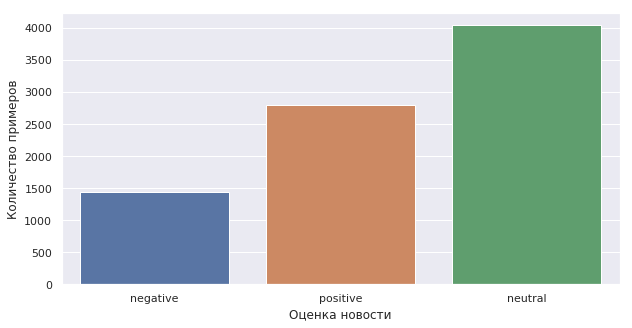
\includegraphics[scale=0.5]{sent_dist}
            \captionof{figure}{Распределение настроения новостей в данных}
        \end{center}

        
    \section{Идеализация модели}
        Откажемся от части информации в данных, которые упростят эксперимент, а также избавимся 
        от выбросов и аномалий. 
        
        Наши ограничения:
        \begin{itemize}
            \item Возьмём из новостей только русские слова
            \item Приведём все слова к нормальной форме через библиотеку pymorphy2\footnote{\href{https://pymorphy2.readthedocs.io}{https://pymorphy2.readthedocs.io}}.
            \item Не будем использовать новостные статьи, где больше 10000 символов
        \end{itemize}

        После данной обработки осталось 7732 статьи.

    \section{Проверка подходов}
        Мы попробуем два метода: 
        
        \textit{Наивный}, который основывается на построении множеств для каждого класса и взвешивания их 
        частоты встречаемости в статьях. 
        
        \textit{Статистический}, преобразуем наши данные так, чтобы можно было 
        воспользоваться статистическими методами, а именно, логистической регрессией.

        Проверять качество моделей будем метрикой F1-score\footnote{\href{https://en.wikipedia.org/wiki/F1\_score}{https://en.wikipedia.org/wiki/F1-score}}

        \subsection{Наивный метод}
            Сначала построим множества слов для каждого класса статей: $S_{neg}$,
            $S_{pos}$, $S_{neu}$ - множества слов из статей с негативной, 
            позитивной и нейтральной меткой, соответственно.

            Построим множества уникальных слов для множеств $S_{neg}$ и $S_{pos}$.
            \begin{center}
                $W_{neg} = S_{neg} / S_{pos}$ и $W_{pos} = S_{pos} / S_{neg}$
            \end{center}

            Пусть $Freq_y(x)$ - функция, которая определяет частоту встречаемости слова $x$
            в множестве $y$. Тогда для оценки настроения новости воспользуемся простым алгоритмом.
            (Algorithm 1). 
            
            \begin{algorithm}[H]
                $sentiment$ = 0

                \For{$word$ \textbf{in} $words$} {
                    \If{$word$ \textbf{in} $W_{pos}$} {
                        $word_{freq}$ = $Freq_{neg}(word)$\\
                        $polarity$ = 1
                    }
                    \If{$word$ \textbf{in} $W_{pos}$} {
                        $word_{freq}$ = $Freq_{pos}(word)$\\
                        $polarity$ = -1
                    }

                    \If{$word$ \textbf{in} $W_{neu}$} {
                        $neutral_{freq}$ = $Freq_{neu}(word)$\\
                        
                        \If{$word_{freq}$ > $\frac{neutral_{freq}}{2}$} {
                            $sentiment$ += $\frac{word_{freq}* polarity}{2}$\\
                            \textbf{continue}
                        }

                        \If{$neutral_{freq}$ > $word_{freq}$} {
                            \textbf{continue}
                        }
                        $sentiment$ += $word_{freq}* polarity$
                    }
                }
                \caption{Оценка настроения новостной статьи}
            \end{algorithm}

            Пройдёмся по всем словам статьи, проверяем имеется ли слово в $W_{pos}$ или $W_{neg}$,
            если да, то сравниваем частоты встречаемости этого слова относительно \textit{Нейтральных}.
            Суммируем все слова статьи и получаем общую оценку настроения статьи.

            Дальше нормируем оценку на количество слов в тексте и подбираем два порога, которые будут
            определять нейтральную часть. 
            
        \subsection{Логистическая регрессия}
            Преобразуем текст в численные значения, чтобы на них обучить логистическую регрессию.

            
            Будем использовать TF-IDF\footnote{\href{https://ru.wikipedia.org/wiki/TF-IDF}{https://ru.wikipedia.org/wiki/TF-IDF}}
            - это статистическая мера оценки важности слова, основываясь на частотах встречаемости слова в тексте и в документе.

            Частота слова $t$ в документе $d$: 
            \begin{center}
                ${{tf} (t,d)={\frac {n_{t}}{\sum _{k}n_{k}}}}$
            \end{center}
            
            Обратная частота документа:
            \begin{center}
                ${idf} (t,D)=\log {\frac {|D|}{|\{\,d_{i}\in D\mid t\in d_{i}\,\}|}}$
            \end{center}

            \textbf{TF-IDF} является произведением двух сомножителей: 
            \begin{center}
                ${tf-idf}(t,d,D) = {tf}(t,d)\times {idf}(t,D)$
            \end{center}

            На самом деле, \textbf{TF-IDF} можно применять не только к одиным словам, но и к нескольким, тем
            самым считая меру важности комбинаций слов, или применять к нескольким символам:
            униграммам, биграммам, триграммам и тд. 

            Мы будем использовать все три статистики, но стоит учесть, что это много информации, в том числе и лишней,
            поэтому мы выберем $N = 30000$ самых часто встречаемых случаев. 

            Тогда текст статьи представляется в виде вектора $news_{vector} \in \mathcal{R}^N$, где по элементам 0, 
            если в тексте нет слова, и tf-idf(слова), если есть.

            На $news_{vector}$ векторах будем строить многоклассовую логистическую регрессию,
            которую называют Softmax Regression\footnote{\href{http://deeplearning.stanford.edu/tutorial/supervised/SoftmaxRegression/}{http://deeplearning.stanford.edu/tutorial/supervised/SoftmaxRegression/}}.

    \section{Эксперименты}
        Наивный метод показал, что он хорошо различает между собой хорошие и плохие новости,
        а вот нейтральные сильно путаются, что видно на распределении нормированной оценки (Рис. 2).
        \begin{center}
            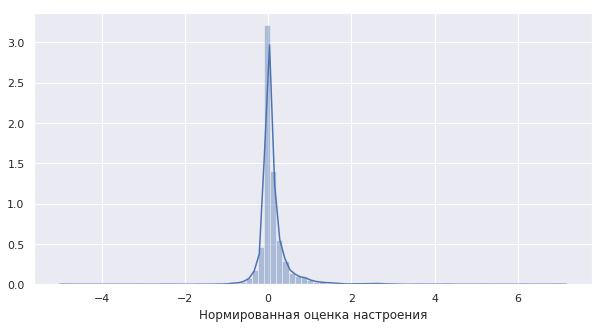
\includegraphics[scale=0.7]{naive_norm}
            \captionof{figure}{Распределение нормированной оценки настроения}
        \end{center}

        Результаты множества слов.
        \begin{itemize}
            \item В хороших словах встречаются такие: делегация, экспедиция, упражнение, наставник, транскаспийский и тд.
            \item В плохих словах: терентьев, оштрафовать, взяточничество, тюремный, вирус, санкционирование и тд.
        \end{itemize}
        
        Подобрали пороговые коэффициенты: если оценка текста выше 0.1, то он позитивный,
        если ниже -0.05, то негативный, иначе нейтральный.

        \begin{center}
            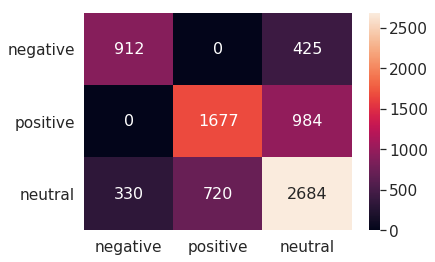
\includegraphics[scale=0.8]{naive_heat}
            \captionof{figure}{Матрица ошибок наивной модели}
        \end{center}

        На матрице ошибок наивного метода (Рис. 3). видно, что модель никогда не путает хорошие новости
        с плохими и наоборот.

        \textbf{Основные метрики по наивной модели}
        \begin{center}
            \begin{tabular}{ c c c c c}
             & precision & recall & f1-score & support\\ 
             negative & 0.73 & 0.68 & 0.71 & 1337\\ 
             neutral & 0.66 & 0.72 & 0.69 & 3734\\
             positive & 0.70 & 0.63 & 0.66 & 2661
            \end{tabular}
        \end{center}

        Логистическая регрессия показала лучше результат, в целом, она распознаёт больше
        статей и меньше ошибается (Рис. 4). В этой модели иногда бывают ошибки между хорошими и плохими 
        новостями, но такие ошибки очень редкие, ими можно пренебречь.

        \begin{center}
            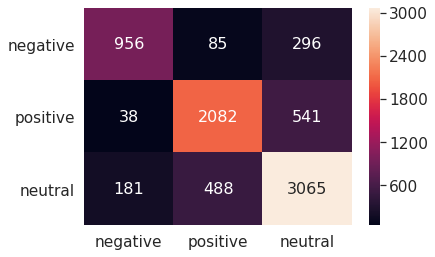
\includegraphics[scale=0.8]{logreg_heat}
            \captionof{figure}{Матрица ошибок многоклассовой логистической регрессии}
        \end{center}

        По матрице ошибок видно, что модель чаще путает позитивные и негативные классы с нейтральными, 
        чем между самими классами. По метрикам модель имеет сильно лучше результат, чем наивный метод.
        
        \textbf{Основные метрики по логистической регрессии}
        \begin{center}
            \begin{tabular}{ c c c c c}
             & precision & recall & f1-score & support\\ 
             negative & 0.89 & 0.82 & 0.85 & 1337\\ 
             neutral & 0.87 & 0.90 & 0.88 & 3734\\
             positive & 0.89 & 0.88 & 0.88 & 2661
            \end{tabular}
        \end{center}

        Код экспериментов находится в открытом доступе\footnote{\href{https://github.com/e1four15f/math-modeling-institute}{https://github.com/e1four15f/math-modeling-institute}}

    \section{Адекватность модели}
        Проверим адекватность модели еще и эмпирически -- найдем и оценим новости с самыми популярными позитивными и негативными словами.

        тут картиначки из news, так нагляднее

        Проверка настроения новостей эмпирическим методом и сравнение моделей доказывает высокую точность определения настроения новостей нашим конечным методом.


\end{document}
